% JUMP TO LINE 60, 75
\documentclass[preview, margin=0.6in]{standalone}
\usepackage[letterpaper,portrait,top=0.4in, left=0.6in, right=0.6in, bottom=1in]{geometry}

\usepackage{amsmath, amsfonts, amsthm, amssymb}
\usepackage{graphicx, float}
\usepackage{mathtools}
\usepackage{titlesec}
\usepackage{interval}
\usepackage{hyperref}
\usepackage{siunitx}
\usepackage{titling}
\usepackage{vwcol}
\usepackage{setspace}
\usepackage{empheq}
\usepackage{cancel}
\usepackage{esdiff}
\usepackage{multicol}
\usepackage{mdframed}
\usepackage{esdiff}
\usepackage{tikzsymbols}
\usepackage{multicol}
\usepackage{tikz}
\usepackage{varwidth}
\usepackage{parskip}
\usepackage{pgfplots}
\usepackage{mlmodern}
\pgfplotsset{compat=1.18}
\intervalconfig {
	soft open fences
}

\newcommand{\alignedintertext}[1]{%
  \noalign{%
    \vtop{\hsize=\linewidth#1\par
    \expandafter}%
    \expandafter\prevdepth\the\prevdepth
  }%
}

\newtheorem{lemma}{Lemma}

\newcommand*{\problem}[1]{\section*{Problem #1}}
\newcommand*{\aps}{\section*{AP Corner}}
\newcommand*{\deriv}[1][x]{\ensuremath{\dfrac{\mathrm{d}}{\mathrm{d}#1}}}
\newcommand*{\floor}[1]{\ensuremath{\lfloor #1\rfloor}}
\newcommand*{\lheqzero}{\ensuremath{\underset{\text{L'H}}{\overset{\left[\frac00\right]}{=}}}}
\newcommand*{\lheqinfty}{\ensuremath{\underset{\text{L'H}}{\overset{\left[\frac{\infty}{\infty}\right]}{=}}}}

\DeclareMathOperator{\DNE}{DNE}
\DeclareMathOperator{\sgn}{sgn}

\DeclareMathOperator{\arccsc}{arccsc}
\DeclareMathOperator{\arcsec}{arcsec}
\DeclareMathOperator{\proj}{proj}
\DeclareMathOperator{\arccot}{arccot}

%opening

\title{\vspace*{-40pt}Classwork Set \#4}
\author{Jayden Li}
\date{\today}
% \allowdisplaybreaks
\postdisplaypenalty=100000

\begin{document}
\setstretch{1.25}
\fontsize{12pt}{12pt}\selectfont
\setlength{\abovedisplayskip}{\abovedisplayskip/2}
\setlength{\belowdisplayskip}{\belowdisplayskip/2}
\setlength{\parindent}{0pt}
\setlength{\parskip}{2ex plus 0.5ex minus 0.2ex}
\maketitle

\problem{2}
$(x,y,z)\cdot(1,2,3)=0$.

\problem{3}
$(x,y,z)$ is in the plane spanned by $u=(3,-1,2)$ and $v=(-1,4,0)$, which means it must be orthogonal to the vector that is orthogonal to both $u$ and $v$. This vector is given by $u\times v$:
\begin{equation*}
    u\times v
	=\begin{vmatrix}
		\hat i & \hat j & \hat k \\
		3 & -1 & 2 \\
		-1 & 4 & 0
	\end{vmatrix}
	=\hat i \left( 0-8 \right)-\hat j \left( 0-(-2) \right)+\hat k \left( 12-1 \right)
	=-8\hat i-2\hat j+11\hat k
	=(-8,-2,11)
\end{equation*}
$(x,y,z)$ is orthogonal to $u\times v=(-8,-2,-11)$ so $(x,y,z)\cdot (-8,-2,-11)=0$.

\problem{4}
We shift the plane by $(1,2,3)$, so it passes through that point instead of the origin $(0,0,0$). This means that $(x-1,y-2,z-3)\cdot (-8,-2,-11)=0$.

\problem{5}

I believe such a line does not exist.

The equation of a line passing through the origin and $(3,-1,2)$ is $(x,y,z)=t(3,-1,2)$. $(-1,4,0)$ is not a scalar multiple of $(3,-1,2)$, so a line passing through these three points cannot exist.

\problem{6}
Line parallel to vector $(-4,5,-2)$ and passing through $(3,-1,2)$. Equivalent to, if $t\in\mathbb R$:
\begin{equation*}
    \begin{bmatrix}
		x \\ y \\ z
    \end{bmatrix}
	=\begin{bmatrix}
		3 \\ -1 \\ 2
	\end{bmatrix}
	+t \begin{bmatrix}
		-4 \\ 5 \\ -2
	\end{bmatrix}
\end{equation*}

\problem{7}

Set each of $(x-x_0)/a,(y-y_0)/b,(z-z_0)/c$ to the parameter $t$ in a set of parametric equations:
\begin{equation*}
	\left\{ 
		\begin{aligned}
			t&=\frac{x-x_0}{a} \\
			t&=\frac{y-y_0}{b} \\
			t&=\frac{z-z_0}{c}
		\end{aligned}
	\right.
	\iff 
	\left\{ 
		\begin{aligned}
			at&=x-x_0 \\
			bt&=y-y_0 \\
			ct&=z-z_0
		\end{aligned}
	\right.
	\iff 
	\left\{ 
		\begin{aligned}
			x&=x_0+at \\
			y&=y_0+bt \\
			z&=z_0+ct
		\end{aligned}
	\right.
	\iff 
	\begin{bmatrix}
		x \\ y \\ z
	\end{bmatrix}
	=\begin{bmatrix}
		x_0 \\ y_0 \\ z_0
	\end{bmatrix}
	+ t\begin{bmatrix}
		a \\ b \\ c
	\end{bmatrix}
\end{equation*}
This is a line passing through the point $(x_0,y_0,z_0)$, and parallel to the vector $(a,b,c)$.

\textit{(I read through the textbook to understand what is going on in questions 6 and 7.)}

\problem{8}

$2x-3y+z=8\iff 2(x-4)-3y+z=0\iff (x-4,y,z)\cdot(2,-3,1)=0$. The plane is orthogonal to $n=(2,-3,1)$.

Let $Q=(Q_x,Q_y,Q_z)$; since $Q$ is on the plane:
\begin{equation*}
    2Q_x-3Q_y+Q_z=8
	\iff Q_z=8-2Q_x+3Q_y
\end{equation*}
From here we have $Q=(Q_x,Q_y,8-2Q_z+3Q_y)$. We also have vector $QP=P-Q$:
\begin{equation*}
    QP=\begin{bmatrix}
		3-Q_x \\
		1-Q_y \\
		7-(8-2Q_x+3Q_y)
    \end{bmatrix}
    =\begin{bmatrix}
		3-Q_x \\
		1-Q_y \\
		-1+2Q_x-3Q_y
    \end{bmatrix}
\end{equation*}
We can calculate the project $\proj_nQP$:
\begin{equation*}
    \proj_nQP 
	=\frac{QP\cdot n}{n\cdot n}n
	=\frac{6-2Q_x-3+3Q_y-1+2Q_x-3Q_y}{2^2+(-3)^2+1^2}n
	=\frac{2}{14}n
	=\boxed{\frac17\begin{bmatrix}
		2 \\ -3 \\ 1
	\end{bmatrix}}
\end{equation*}

\problem{9}

$\lVert \proj_n QP \rVert $ is the shortest distance between the plane and $P$.
\begin{center}
	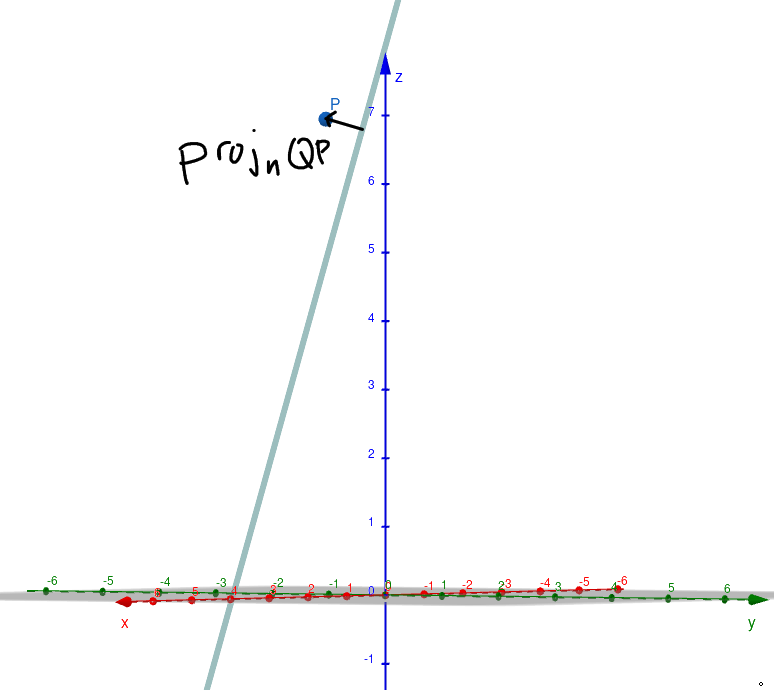
\includegraphics[width=0.6\linewidth]{q9.png}
\end{center}

\begin{mdframed}
	We can also do this another way to verify this answer. We can find the projection of $P$ onto the plane, and calculate the error. This error should equal $\proj_nQP=(2,-3,1)/7$.

	First, we shift everything for convenience. Instead of projecting $P$ onto the plane, we project $P'=P-(4,0,0)=(-1,1,7)$ onto the plane formed by $2x-3y+z=0$, or:
	\begin{equation*}
	    \begin{bmatrix}
			2 & -3 & 1
	    \end{bmatrix}
		\begin{bmatrix}
			x \\ y \\ z
		\end{bmatrix}
		=0
		\iff 
	    \begin{bmatrix}
			1 & -\dfrac32 & \dfrac12
	    \end{bmatrix}
		\begin{bmatrix}
			x \\ y \\ z
		\end{bmatrix}
		=0
	\end{equation*}
	So this plane is spanned by vectors $(3/2,1,0)$ and $(-1/2,0,1)$, and a vector $v$ is in the plane if and only if $v\in C(A)$:
	\begin{equation*}
		A=\begin{pmatrix}
			3/2 & -1/2 \\
			1 & 0 \\ 
			0 & 1
		\end{pmatrix}
	\end{equation*}
	We project onto the column space of $A$, which is the plane. To project the point $P'=(-1,1,7)$, we calculate $R=A(A^TA)^{-1}A^TP'$, and the error of the projection is $P'-R$.

	Calculator says the error $P'-R=P'-A(A^TA)^{-1}A^TP'=(2,-3,1)/7$. Great.
\end{mdframed}


\end{document}
